\documentclass[conference]{IEEEtran}
\IEEEoverridecommandlockouts
\usepackage{cite}
\usepackage{amsmath,amssymb,amsfonts}
\usepackage{algorithmic}
\usepackage{algorithm}
\usepackage{graphicx}
\usepackage{textcomp}
\usepackage{xcolor}
\usepackage{booktabs}
\usepackage{multirow}
\usepackage{subcaption}
\usepackage{flushend}
\usepackage{tikz}
\usetikzlibrary{arrows.meta}
% Use Times-like font when available (compatible with pdflatex and xelatex)
\usepackage{iftex}
\ifPDFTeX
  \IfFileExists{newtxtext.sty}{\usepackage{newtxtext,newtxmath}}{}
\else
  \usepackage{fontspec}
  \IfFontExistsTF{Times New Roman}{\setmainfont{Times New Roman}}{}
\fi

\graphicspath{{../analysis_output/}}

\def\BibTeX{{\rm B\kern-.05em{\sc i\kern-.025em b}\kern-.08em
    T\kern-.1667em\lower.7ex\hbox{E}\kern-.125emX}}
\begin{document}

\title{The Good Plate: A Self-Stabilizing Adaptive\\
  Tray as a Real-Time Cyber-Physical System}

\author{
\IEEEauthorblockN{Zhen-Rong Wu}
\IEEEauthorblockA{\textit{Dept. of Computer Science}\\
\textit{and Information Engineering}\\{National Taiwan Normal University} \\
41247012S@ntnu.edu.tw}
\and
\IEEEauthorblockN{Darrin Lin}
\IEEEauthorblockA{\textit{Dept. of Computer Science}\\
\textit{and Information Engineering}\\{National Taiwan Normal University} \\
41247022S@ntnu.edu.tw}
\and
\IEEEauthorblockN{Xin-Shao Hon}
\IEEEauthorblockA{\textit{Dept. of Computer Science}\\
\textit{and Information Engineering} \\{National Taiwan Normal University} \\
41247033S@ntnu.edu.tw}
}

\maketitle

\begin{abstract}
  This paper presents \emph{The Good Plate}, a self-stabilizing adaptive tray that keeps
  its top surface level despite external tilting disturbances, so that objects
  placed on it do not slide or topple. The platform is supported by a central
  universal joint and actuated by four MG90S servos that reel four strings
  attached to the platform corners. A GY-521/MPU6050 inertial measurement unit
  (IMU) senses the tilt, a complementary filter fuses its accelerometer and
  gyroscope into a drift-free attitude estimate, and two independent
  velocity-form proportional--integral (PI) controllers drive the pitch and roll
  angles toward zero. A key contribution is an exact inverse-kinematic model that
  converts a desired tilt angle into the precise string length each servo must
  produce, derived from first principles using a rigid-body rotation of the
  platform about the joint; this replaces the naive ``servo-angle equals
  tilt-angle'' mapping, which is strongly nonlinear and fails in practice. The
  firmware runs a closed loop at \mbox{500\,Hz} on an STM32F401 microcontroller.
  Using on-chip cycle-accurate timing across $36{,}031$ control cycles, the
  task set is shown to be provably schedulable ($\sum_i C_i = 1629\,\mu\text{s} \le D =
    2000\,\mu\text{s}$) with \mbox{0.00\%} deadline misses. Because the controller
  omits an explicit rate-damping term, the Lyapunov derivative cannot be signed
  analytically; stability is therefore certified \emph{quantitatively from logged
    data} using two complementary measures---the exponential decay rate $\gamma$ of
  the energy envelope and the fraction of samples for which $\dot V \le 0$. The
  data show a bounded, decaying energy ($\gamma = 0.275\,\text{s}^{-1}$) that
  settles into a $\sim\!3.4^\circ$ residual ball, establishing
  \emph{practical (ultimately bounded) stability}.
\end{abstract}

\begin{IEEEkeywords}
  cyber-physical systems, self-stabilization, complementary filter, PID control,
  inverse kinematics, real-time scheduling, Lyapunov stability, STM32, MPU6050.
\end{IEEEkeywords}

% =====================================================
\section{Introduction}
% =====================================================
Carrying a tray of objects---cups, plates, instruments---is a task humans
perform by continuously adjusting the tray angle to keep it level. This work aims
to automate this reflex: an \emph{adaptive tray} that, when tilted by an
external disturbance (a bumped table, a vibrating surface, a hand carrying it
unevenly), re-levels itself fast enough that objects resting on it do not slide
off. This is a canonical cyber-physical system (CPS): a tight loop in which
physical sensing, embedded computation, and physical actuation are
co-designed and must meet real-time deadlines to be correct.

Rather than building a fully enclosed tray, the underlying
\emph{self-stabilizing platform} was developed. The platform rests on
a single central universal joint that bears the load and allows two rotational
degrees of freedom (pitch and roll). Four strings, attached to the four
platform corners and wound on four servo spools, set the platform attitude by
reeling string in or paying it out. The mechanism is shown in
Fig.~\ref{fig:hardware}.

The contributions of this paper are:
\begin{enumerate}
  \item A complete embedded CPS pipeline---IMU $\rightarrow$ complementary
        filter $\rightarrow$ velocity-form PI $\rightarrow$ string-length
        inverse kinematics $\rightarrow$ PWM---running closed-loop at 500\,Hz on
        a single STM32F401.
  \item An \emph{exact} string-length model (Section~\ref{sec:geometry})
        derived from a rigid-body rotation about the joint, including the
        often-neglected upper-pillar offset, and its conversion to a servo
        angle through the spool circumference.
  \item A formal and empirical real-time schedulability analysis based on
        on-chip cycle-counter measurements (Section~\ref{sec:rt}).
  \item A \emph{data-driven} Lyapunov stability argument
        (Section~\ref{sec:lyap}) that, in the absence of an explicit damping
        term and an identified plant model, certifies practical stability
        through two quantitative measures, the decay rate $\gamma$ and the
        $\dot V \le 0$ fraction.
\end{enumerate}

% =====================================================
\section{System Architecture}
% =====================================================
\begin{figure}[t]
  \centering
  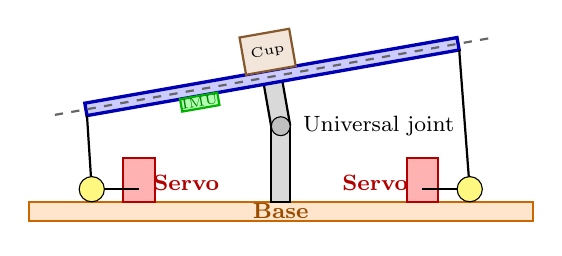
\begin{tikzpicture}[scale=0.8, every node/.style={font=\footnotesize}]
    % Base
    \draw[fill=orange!20, draw=orange!80!black, thick]
    (-4, -1.5) rectangle (4, -1.2);
    \node[text=orange!60!black] at (0, -1.35) {\textbf{Base}};

    % Central pillar (lower part)
    \draw[fill=gray!30, draw=black, thick]
    (-0.15, -1.2) rectangle (0.15, 0);
    \node[anchor=west] at (0.2, 0)
    {Universal joint};



    % Horizontal reference line (level baseline)
    % Rotated upper system around universal joint (0,0)
    \begin{scope}[rotate around={10:(0, 0)}]
      % Upper central pillar
      \draw[fill=gray!30, draw=black, thick] (-0.15, 0) rectangle (0.15, 0.8);
      % Platform
      \draw[fill=blue!20, draw=blue!70!black, very thick] (-3, 0.7) rectangle (3, 0.9);
      \draw[dashed, black!60, thick] (-3.5, 0.8) -- (3.5, 0.8);
      \coordinate (P_L) at (-3, 0.7);
      \coordinate (P_R) at (3, 0.7);
      % Cup
      \draw[fill=brown!20, draw=brown!70!black, thick] (-0.4, 0.9) rectangle (0.4, 1.5);
      \node[rotate=10] at (0, 1.2) {\tiny Cup};
      % IMU
      \draw[fill=green!30, draw=green!70!black, thick] (-1.5, 0.5) rectangle (-0.9, 0.7);
      \node[rotate=10, text=green!50!black] at (-1.2, 0.6) {\tiny IMU};
    \end{scope}
    % Joint sphere
    \draw[fill=gray!50, draw=black] (0, 0) circle (0.15);

    % Servos (left and right)
    \draw[fill=red!30, draw=red!70!black, thick]
    (-2, -1.2) rectangle (-2.5, -0.5);
    \draw[fill=red!30, draw=red!70!black, thick] (2.0, -1.2) rectangle (2.5, -0.5);
    \node[text=red!70!black] at (-1.5, -0.9) {\textbf{Servo}};
    \node[text=red!70!black] at (1.5, -0.9) {\textbf{Servo}};

    % Strings (connected to rotated platform endpoints)
    \draw[black, thick] (P_L) -- (-3, -1.0);
    \draw[black, thick] (P_R) -- (3, -1.0);
    \draw[black, thick] (-3, -1.0) -- (-2.25, -1.0);
    \draw[black, thick] (3, -1.0) -- (2.25, -1.0);

    % Pulleys
    \draw[fill=yellow!50, draw=black] (-3, -1.0) circle (0.2);
    \draw[fill=yellow!50, draw=black] (3, -1.0) circle (0.2);

    % Annotations
    % \node[anchor=west, text=accentblue] at (3.5, 0.5) {$\theta$ tilt};
  \end{tikzpicture}
  \caption{Mechanical structure (one axis shown). The platform rests on a central
    universal joint that bears the load; four strings on servo-driven spools pull
    the four corners. Cross-pairs act antagonistically: one reels in while the
    opposite pays out. The IMU rides on the platform.}
  \label{fig:hardware}
\end{figure}

\subsection{Hardware}
The platform (Fig.~\ref{fig:hardware}) consists of:
\begin{itemize}
  \item \textbf{MCU:} STM32F401CCU6 (Arm Cortex-M4F at 84\,MHz).
  \item \textbf{IMU:} GY-521 module carrying an InvenSense MPU6050
        (3-axis accelerometer $+$ 3-axis gyroscope) on the platform, read over
        I\textsuperscript{2}C at 100\,kHz.
  \item \textbf{Actuators:} $4\times$ MG90S hobby servos, each driving a spool
        that winds one string; PWM at 50\,Hz from a single TIM2 with four
        compare channels.
  \item \textbf{Mechanism:} a central universal joint carries the platform
        load; the four strings only \emph{steer} the attitude. Cross-pairs act
        \emph{antagonistically}---to tilt one way, one string reels in while
        the opposite one pays out.
\end{itemize}

\begin{figure}[t]
  \centering
  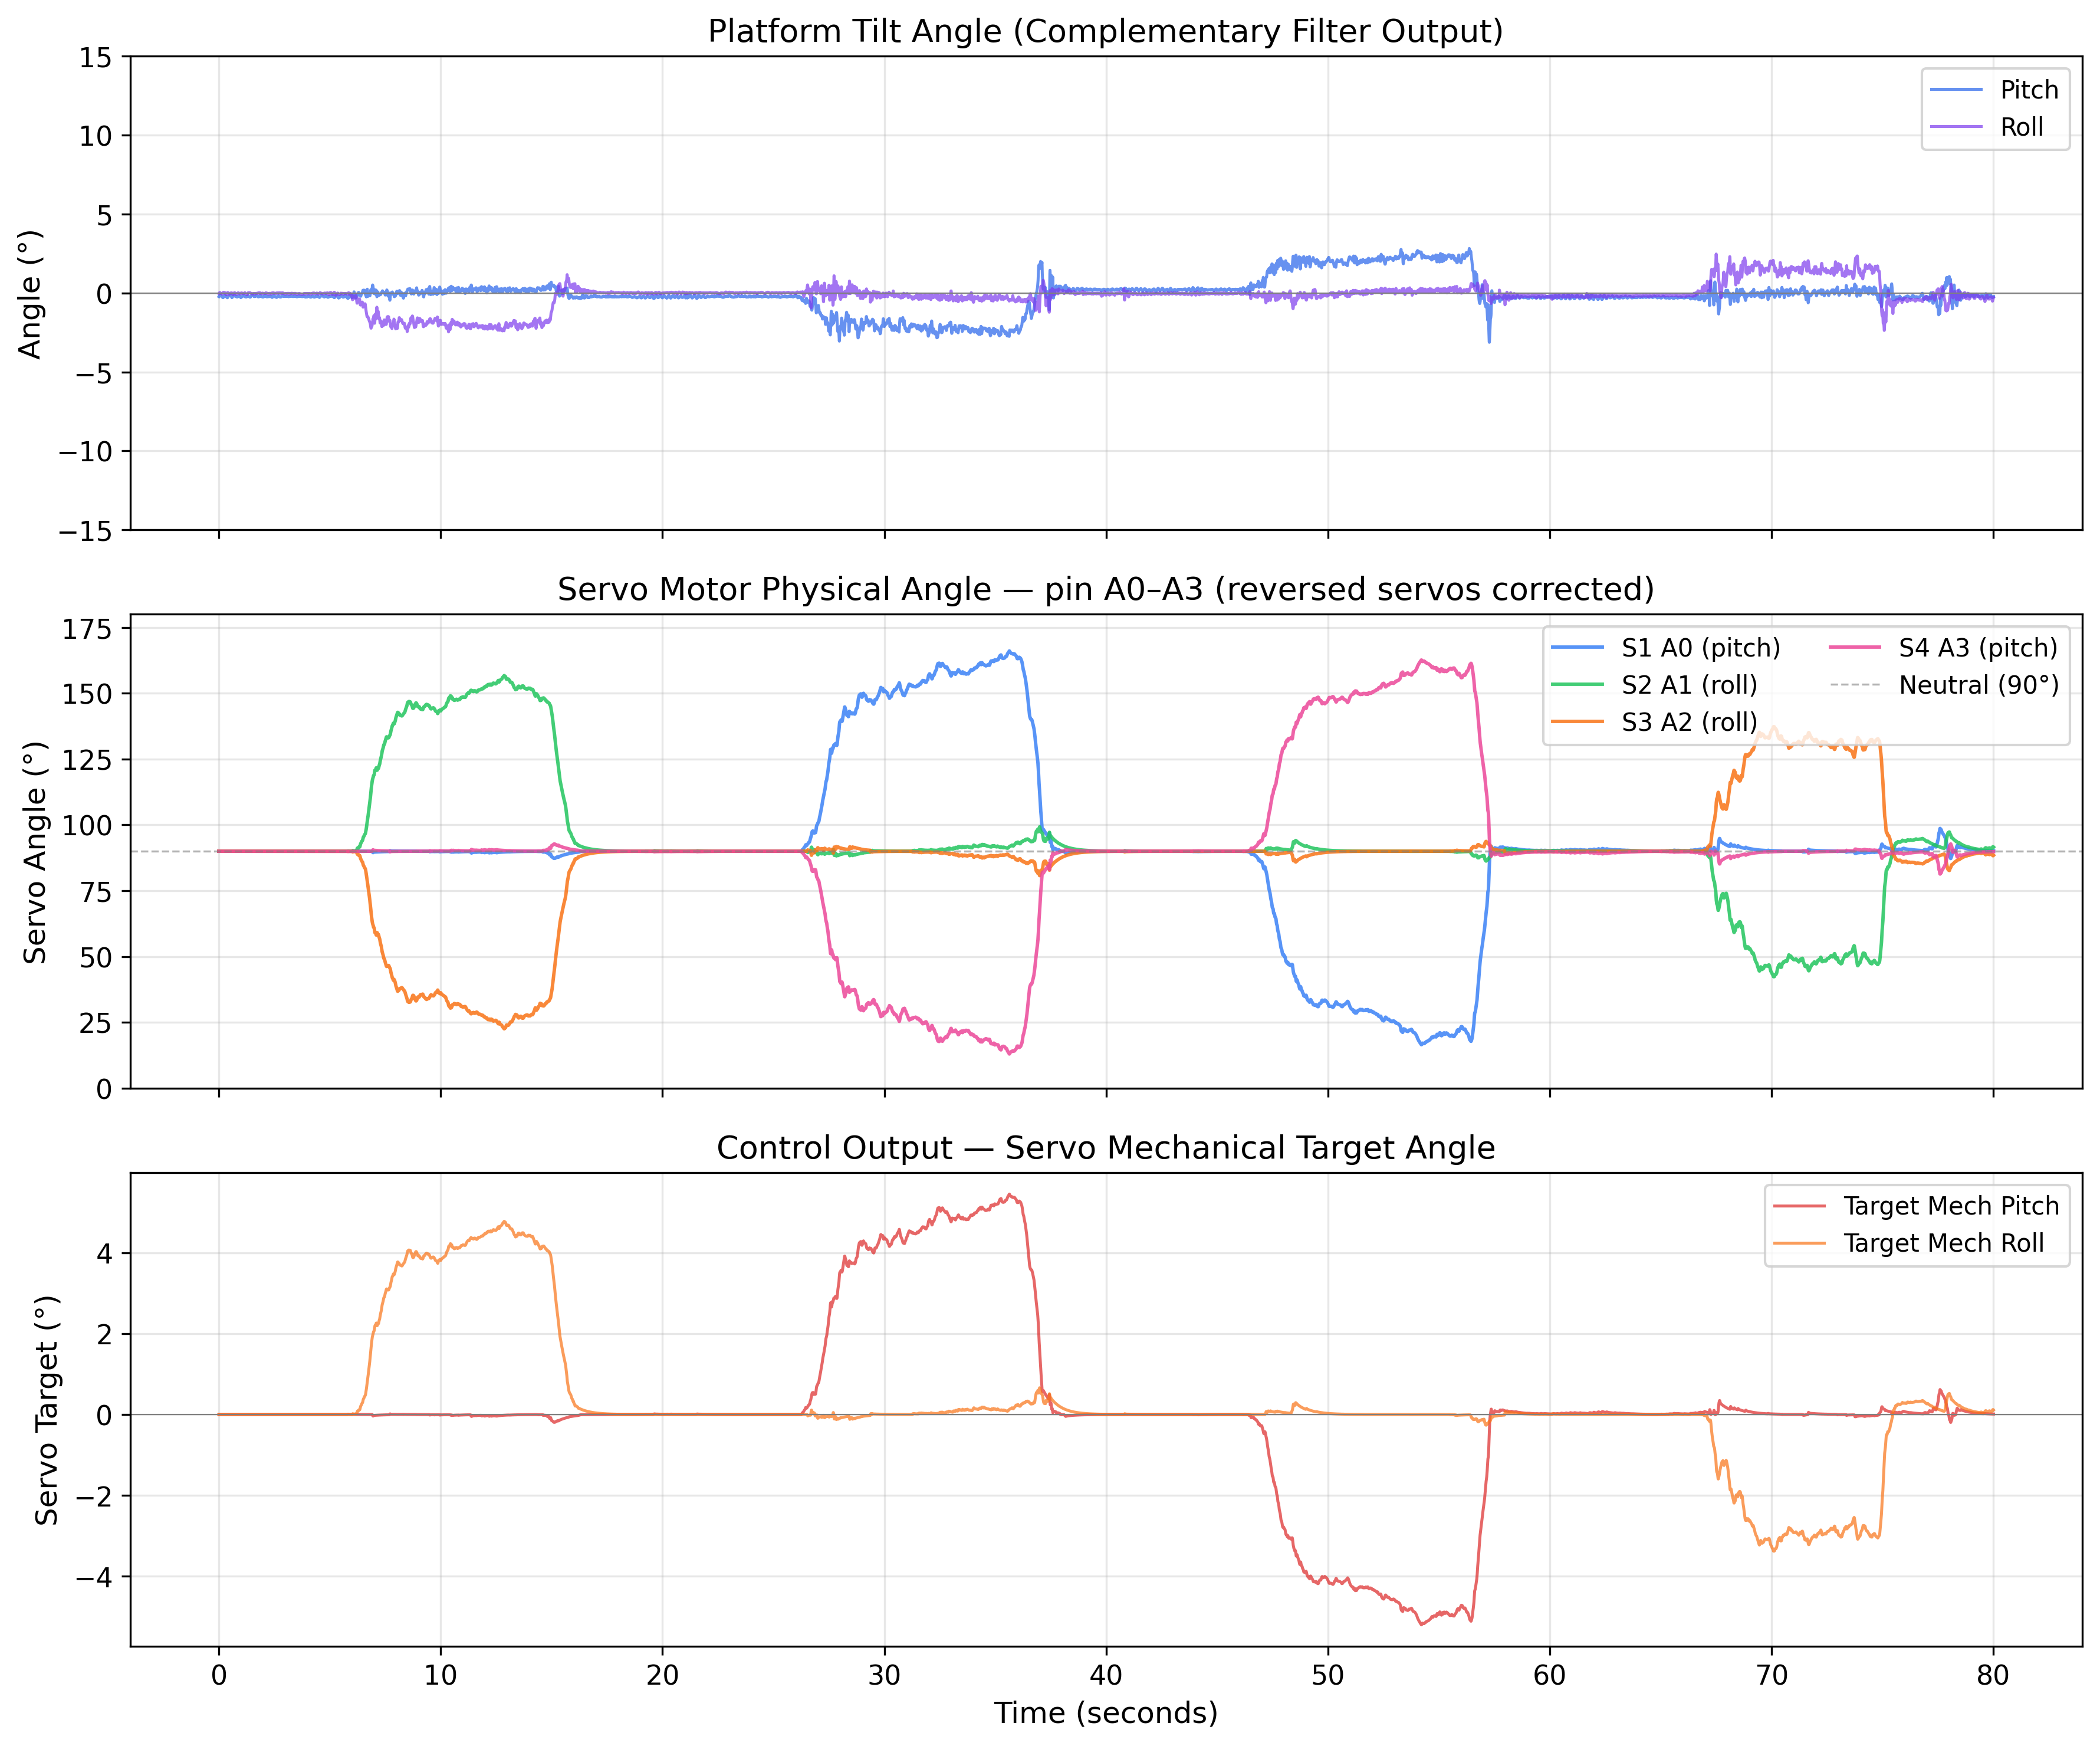
\includegraphics[width=0.92\linewidth]{fig5_control_signal.png}
  \caption{Top-to-bottom: measured platform tilt (complementary-filter output),
    the four servos' physical angles (pin order A0--A3, with the two
    mechanically-reversed servos corrected), and the controller's accumulated
    mechanical target angle. The antagonistic action is visible: when one servo
    of a pair rises above the $90^\circ$ neutral, its partner falls below it.}
  \label{fig:controlsignal}
\end{figure}

\subsection{Signal flow}
Each control cycle executes five tasks in a fixed sequence:
\[
  \underbrace{\text{IMU read}}_{\tau_1}\rightarrow
  \underbrace{\text{comp.\ filter}}_{\tau_2}\rightarrow
  \underbrace{\text{PI control}}_{\tau_3}
\]
\[
  \rightarrow
  \underbrace{\text{cable geometry}}_{\tau_4}
  \rightarrow
  \underbrace{\text{servo PWM}}_{\tau_5}.
\]
Pitch and roll are controlled by two independent single-input single-output
loops; all computation, logging (over USB-CDC), and timing instrumentation run
on the STM32F401 within one $2\,\text{ms}$ period.

% =====================================================
\section{Attitude Estimation}
% =====================================================
\subsection{What the MPU6050 measures}
The accelerometer measures \emph{specific force} (in $g$): even at rest it reads
$+1g$ along the axis opposing gravity, because the proof mass's spring reacts to
gravity, $\vec a_\text{meas} = \vec a_\text{motion} - \vec g$. The gyroscope
measures angular rate (in deg/s). Raw 16-bit samples are scaled by the
configured sensitivities ($16384\,\text{LSB}/g$ at $\pm2g$,
$131\,\text{LSB}/(\text{deg/s})$ at $\pm250\,\text{deg/s}$) and de-biased using
offsets captured at startup, where the platform is held flat and still and 500
samples are averaged (the $z$-axis offset is referenced to $+1g$).

From the accelerometer alone, the instantaneous tilt angles are
\begin{equation}
  \theta_p^\text{acc} = \operatorname{atan2}\!\big(a_y,\,a_z\big),\quad
  \theta_r^\text{acc} = -\operatorname{atan2}\!\Big(\!-a_x,\,\sqrt{a_y^2+a_z^2}\Big).
\end{equation}

\subsection{Complementary filter}
Neither sensor is sufficient alone: the accelerometer is accurate at low
frequency (gravity is a stable reference) but is corrupted by inertial
acceleration during motion; the gyroscope is accurate at high frequency but its
integrated angle drifts over time. They are fused with a fixed-weight
\emph{complementary filter}~\cite{higgins1975comparison,colton2007balance},
which high-passes the gyro and low-passes the accelerometer so the two transfer
functions sum to unity gain:
\begin{equation}
  \boxed{\;\hat\theta_k = \alpha\big(\hat\theta_{k-1} + \omega_k\,\Delta t\big)
    + (1-\alpha)\,\theta_k^\text{acc}\;}
  \label{eq:compfilter}
\end{equation}
with $\alpha = 0.96$ and $\Delta t$ the measured loop period. The gyro axes map
as $\texttt{gy}\!\rightarrow\!\text{pitch}$ and
$\texttt{gx}\!\rightarrow\!\text{roll}$. A Kalman filter would adapt the weights
online, but the fixed-weight form is sufficient for the low-speed platform and
costs only one multiply and one add per axis (Table~\ref{tab:tasks}). The parameter
$\alpha$ is deliberately kept high to favor the gyro short-term and let the
accelerometer correct drift only slowly, which suppresses vibration artifacts.

% =====================================================
\section{Control Design}
% =====================================================
\subsection{Problem statement}
With reference $\theta_\text{ref}=0$, the error on each axis is
$e(t) = \theta_\text{ref}-\theta(t) = -\theta(t)$. The objective is to design a control law that
reacts quickly to disturbances, rejects steady offsets (e.g.\ when the whole
base is tilted), and avoids overshoot. The classical answer is the PID
controller~\cite{astrom1995pid,ogata2010modern}:
\begin{equation}
  u(t) = K_p\,e(t) + K_i\!\int_0^t\! e(\tau)\,d\tau + K_d\,\frac{de(t)}{dt}.
\end{equation}

\subsection{Velocity (incremental) form}
Discretizing with a rectangular integral and a backward-difference derivative
and then differencing consecutive outputs, $u_k - u_{k-1}$, yields the
\emph{velocity form}:
\begin{equation}
  \Delta u_k = K_p\,[e_k-e_{k-1}] + K_i\,\Delta t\, e_k
  + \frac{K_d}{\Delta t}\,[e_k-2e_{k-1}+e_{k-2}].
\end{equation}
The second difference in the derivative term is extremely sensitive to sensor
noise on a microcontroller. Therefore, $K_d$ is dropped and a
\textbf{velocity-form PI} is implemented:
\begin{equation}
  \boxed{\;\Delta u_k = K_{P}\,[e_k-e_{k-1}] + K_{I}\, e_k\;}
  \label{eq:velpi}
\end{equation}
with $K_{P}=0.1$, $K_{I}=0.01$ in the firmware. The controller output is the
\emph{accumulated} target mechanical angle $u_k=\sum_{j\le k}\Delta u_j$, which
is exactly the integrator state. Accumulating \eqref{eq:velpi} telescopes the
first-difference term and recovers the positional law,
\begin{equation}
  u_k=\sum_{j=0}^{k}\Delta u_j = K_{P}\,e_k + K_{I}\sum_{j=0}^{k}e_j,
\end{equation}
so $K_{P}$ plays the role of the \emph{proportional} action and $K_{I}$ that of
the \emph{integral} action---the velocity form is mathematically equivalent to a
positional PI while being numerically gentler. To suppress residual noise on the
first difference, $[e_k-e_{k-1}]$ is passed through a one-pole low-pass
($\beta=0.85$) before use.

\subsection{Practical safeguards}
Four mechanisms make \eqref{eq:velpi} robust on real hardware:
\begin{itemize}
  \item \textbf{Soft deadband.} Errors below $0.3^\circ$ are zeroed (with a
        continuous, offset-subtracting shaping so there is no jump at the edge),
        preventing servo chatter around level.
  \item \textbf{Leaky integrator.} A term $-\lambda\,u_k$ ($\lambda=0.004$) is
        added to $\Delta u_k$, slowly pulling the accumulated command back
        toward zero. This bleeds off integrator wind-up and self-excitation at
        the cost of a small steady-state residual.
  \item \textbf{Adaptive slew limit.} The per-cycle step $|\Delta u_k|$ is
        clamped to a bound that grows with the error magnitude
        ($0.12^\circ$ for $<\!4^\circ$ up to $0.6^\circ$ for $>\!20^\circ$),
        giving fast recovery for large disturbances and gentle, overshoot-free
        motion near level.
  \item \textbf{Conditional-integration anti-windup.} Before committing a step,
        the firmware computes the resulting servo command; if it would exceed
        the physical $[0^\circ,180^\circ]$ range (or the $\pm50^\circ$
        mechanical tilt limit), the step is \emph{rejected} and the integrator
        holds. Once the disturbance clears, the platform re-levels with no
        wind-up lag.
\end{itemize}

% =====================================================
\section{String-Length Geometry (Inverse Kinematics)}
\label{sec:geometry}
% =====================================================
The PI controller outputs a desired tilt \emph{angle}, but each servo controls
the \emph{length of a string}. A naive mapping---increment the servo angle by
the angle error---fails because one degree of servo rotation does not produce one
degree of platform tilt: the relationship is strongly nonlinear, since the
strings connect a rotating platform to fixed servo positions. Instead, the \emph{exact}
string length required at the desired tilt is computed and converted to a servo rotation.
The geometry (per axis) is shown in
Fig.~\ref{fig:geometry}.

\begin{figure}[t]
  \centering
  \begin{minipage}{\linewidth}
    \centering
    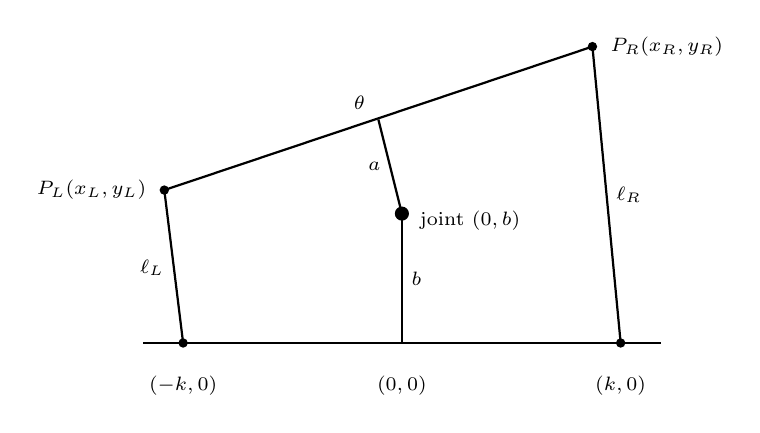
\begin{tikzpicture}[x=0.85pt, y=0.85pt, every node/.style={font=\footnotesize}]
      % base line
      \draw[thick] (0,20) -- (220,20);
      % servos
      \fill (17,20) circle (2);
      \fill (203,20) circle (2);
      \node[below] at (17,10) {\scriptsize $(-k,0)$};
      \node[below] at (203,10) {\scriptsize $(k,0)$};
      \node[below] at (110,10) {\scriptsize $(0,0)$};
      % lower pillar b
      \draw[thick] (110,20) -- (110,75);
      \node[right] at (110,47.5) {\scriptsize $b$};
      % joint
      \fill (110,75) circle (3);
      \node[right=3pt] at (110,72) {\scriptsize joint $(0,b)$};
      % upper pillar a (tilted)
      \draw[thick] (110,75) -- (100,115);
      \node[left] at (105,95) {\scriptsize $a$};
      % platform
      \draw[thick] (9,85) -- (191,146);
      \fill (9,85) circle (2);
      \fill (191,146) circle (2);
      \node[left=3pt] at (9,85) {\scriptsize $P_L(x_L, y_L)$};
      \node[right=3pt] at (191,146) {\scriptsize $P_R(x_R, y_R)$};
      % strings (slanted)
      \draw[black, thick] (9,85) -- (17,20);
      \draw[black, thick] (191,146) -- (203,20);
      \node[left] at (13,52) {\scriptsize $\ell_L$};
      \node[right] at (197,83) {\scriptsize $\ell_R$};
      % theta label
      \node at (92,122) {\scriptsize $\theta$};
    \end{tikzpicture}
  \end{minipage}
  \caption{Per-axis geometry. The platform tilts by $\theta$ about the universal
    joint at $(0,b)$. A rigid upper pillar of length $a$ ties the joint to the
    platform center, so it rotates with the platform. Strings of length
    $\ell_L,\ell_R$ run from the platform ends (offset $\pm k$) to fixed servos at
    $(\pm k,0)$.}
  \label{fig:geometry}
\end{figure}

\subsection{Step 1: locate the platform center}
The platform pivots about the joint at $(0,b)$. A rigid \emph{upper pillar} of
length $a$ connects the joint to the platform center, so the center rotates with
the platform. At rest, the center sits at $(0,b+a)$; its offset from the joint
is the vector $(0,a)^\top$. Rotating that offset by $\theta$ with the standard
planar rotation matrix,
\begin{equation}
  \text{offset}' =
  \begin{bmatrix}\cos\theta & -\sin\theta\\ \sin\theta & \cos\theta\end{bmatrix}
  \begin{bmatrix}0\\ a\end{bmatrix}
  = \begin{bmatrix}-a\sin\theta\\ a\cos\theta\end{bmatrix},
\end{equation}
and adding back the joint position $(0,b)$ gives
\begin{equation}
  \boxed{\;P_\text{center} = \big(-a\sin\theta,\; b + a\cos\theta\big).\;}
\end{equation}
Keeping the $a$ term is what distinguishes the proposed model from a naive single-pillar
setup: because $a$ is not negligible relative to $k$, dropping it introduces a
center-position error of up to $a\sin\theta_{\max}$.

\subsection{Step 2: platform endpoints and string lengths}
Each platform end is offset $\pm k$ \emph{along} the platform. After the same
rotation, those offsets become $(\pm k\cos\theta,\ \pm k\sin\theta)$. Adding them
to $P_\text{center}$:
\begin{align}
  P_R & = \big(-a\sin\theta + k\cos\theta,\; b + a\cos\theta + k\sin\theta\big), \\
  P_L & = \big(-a\sin\theta - k\cos\theta,\; b + a\cos\theta - k\sin\theta\big).
\end{align}
The string length is the Euclidean distance from each endpoint to its servo at
$(\pm k,0)$, $\ell_R = \lVert P_R-(k,0)\rVert$,
$\ell_L = \lVert P_L-(-k,0)\rVert$, i.e.
\begin{align}
  \ell_R(\theta) & = \sqrt{(-a\sin\theta + k\cos\theta - k)^2
    + (b + a\cos\theta + k\sin\theta)^2},
  \label{eq:lr}                                               \\
  \ell_L(\theta) & = \sqrt{(-a\sin\theta - k\cos\theta + k)^2
    + (b + a\cos\theta - k\sin\theta)^2}.
  \label{eq:ll}
\end{align}
These are exactly the expressions evaluated by the firmware routine
\texttt{calculateTargets()}.

\subsection{Sanity check at $\theta=0$}
Substituting $\sin0=0,\ \cos0=1$ into \eqref{eq:lr}--\eqref{eq:ll},
\begin{equation}
  \ell_R(0)=\sqrt{(k-k)^2+(b+a)^2}=a+b,\quad \ell_L(0)=a+b,
\end{equation}
so both strings have the neutral length $a+b$ when level, as required. Subsequent calculations
utilize the length \emph{change} relative to neutral,
$\Delta\ell_{R,L}(\theta) = \ell_{R,L}(\theta) - (a+b)$.

\paragraph{Numerical example} With the measured constants
$a=2.2$, $b=4.5$, $k=11.4$ (cm) and $\theta=10^\circ$,
\begin{align*}
  \ell_R(10^\circ) & \approx 8.66\,\text{cm}\;(\Delta\ell_R\approx+1.96\,\text{cm, pay out}), \\
  \ell_L(10^\circ) & \approx 4.69\,\text{cm}\;(\Delta\ell_L\approx-2.01\,\text{cm, reel in}).
\end{align*}
The two strings move \emph{antagonistically}---one shortens while the other
lengthens---which is precisely the behavior visible in
Fig.~\ref{fig:controlsignal}.

\subsection{Step 3: string length to servo angle}
A servo spool of circumference $C$ winds one full $C$ of string per $360^\circ$
revolution, so the servo rotation $\alpha$ that produces a length change
$\Delta\ell$ is
\begin{equation}
  \Delta\ell = C\cdot\frac{\alpha}{360^\circ}
  \;\Longrightarrow\;
  \boxed{\;\alpha=\frac{360^\circ\,\Delta\ell}{C}.\;}
  \label{eq:alpha}
\end{equation}
The firmware computes the \emph{absolute} angle $\alpha=360^\circ\ell/C$ for both
the live tilt and (once, at boot) for $\theta=0$, storing the latter as
$\alpha_\text{base}$. The PWM command for a standard $0$--$180^\circ$ servo whose
neutral is $90^\circ$ is then
\begin{equation}
  \theta_\text{servo} = 90^\circ + (\alpha - \alpha_\text{base})
  = 90^\circ + \frac{360^\circ\,\Delta\ell}{C},
\end{equation}
with the sign inverted for the two mechanically-reversed servos. With $C=5.1$\,cm
in this implementation, the $\Delta\ell_R=+1.96$\,cm of the example maps to a servo
rotation of $\alpha\approx138^\circ$; a larger spool circumference trades range
for finer resolution.

\subsection{Full pipeline}
Per axis and per cycle: (1) read IMU and estimate $\theta_p,\theta_r$ via
\eqref{eq:compfilter}; (2) update the velocity-form PI \eqref{eq:velpi} to get
the target mechanical angles; (3) evaluate \eqref{eq:lr}--\eqref{eq:ll} for the
required string lengths; (4) map each to a servo angle via \eqref{eq:alpha}; and
(5) emit PWM on the four TIM2 channels. The same procedure runs for both axes
within one $2\,\text{ms}$ period.

% =====================================================
\section{Real-Time Schedulability}
\label{sec:rt}
% =====================================================
\subsection{Task model}
The five tasks form a single-rate, non-preemptive sequential chain
$\tau_1\!\rightarrow\!\tau_2\!\rightarrow\!\tau_3\!\rightarrow\!\tau_4\!\rightarrow\!\tau_5$
with a common control period and implicit deadline $T = D = 2000\,\mu\text{s}$
(500\,Hz). Each task was instrumented with the Cortex-M4 Data Watchpoint and
Trace (DWT) cycle counter~\cite{arm2010cortexm4} (at 84\,MHz, $1\,\mu\text{s} =
84$ cycles), and $36{,}031$ cycles were logged. The per-task statistics are listed in
Table~\ref{tab:tasks}, and a representative timing diagram is shown in
Fig.~\ref{fig:timing}.

\begin{table}[t]
  \caption{Measured Task Execution Times ($N=36{,}031$ cycles)}
  \label{tab:tasks}
  \centering
  \small
  \begin{tabular}{llrrrr}
    \toprule
             & \textbf{Task}                    & \textbf{Mean} & \textbf{P99} & \textbf{WCET} & \textbf{Util.}  \\
             &                                  & ($\mu$s)      & ($\mu$s)     & ($\mu$s)      &                 \\
    \midrule
    $\tau_1$ & IMU read (I\textsuperscript{2}C) & 1558          & 1558         & 1573          & 78.6\%          \\
    $\tau_2$ & Complementary filter             & 6             & 6            & 7             & 0.4\%           \\
    $\tau_3$ & PI control                       & 2             & 3            & 3             & 0.1\%           \\
    $\tau_4$ & Cable geometry                   & 31            & 41           & 42            & 2.1\%           \\
    $\tau_5$ & Servo PWM update                 & 0             & 2            & 4             & 0.2\%           \\
    \midrule
             & \textbf{Total}                   & 1597          & ---          & \textbf{1629} & \textbf{81.5\%} \\
    \bottomrule
  \end{tabular}
\end{table}

\begin{figure}[t]
  \centering
  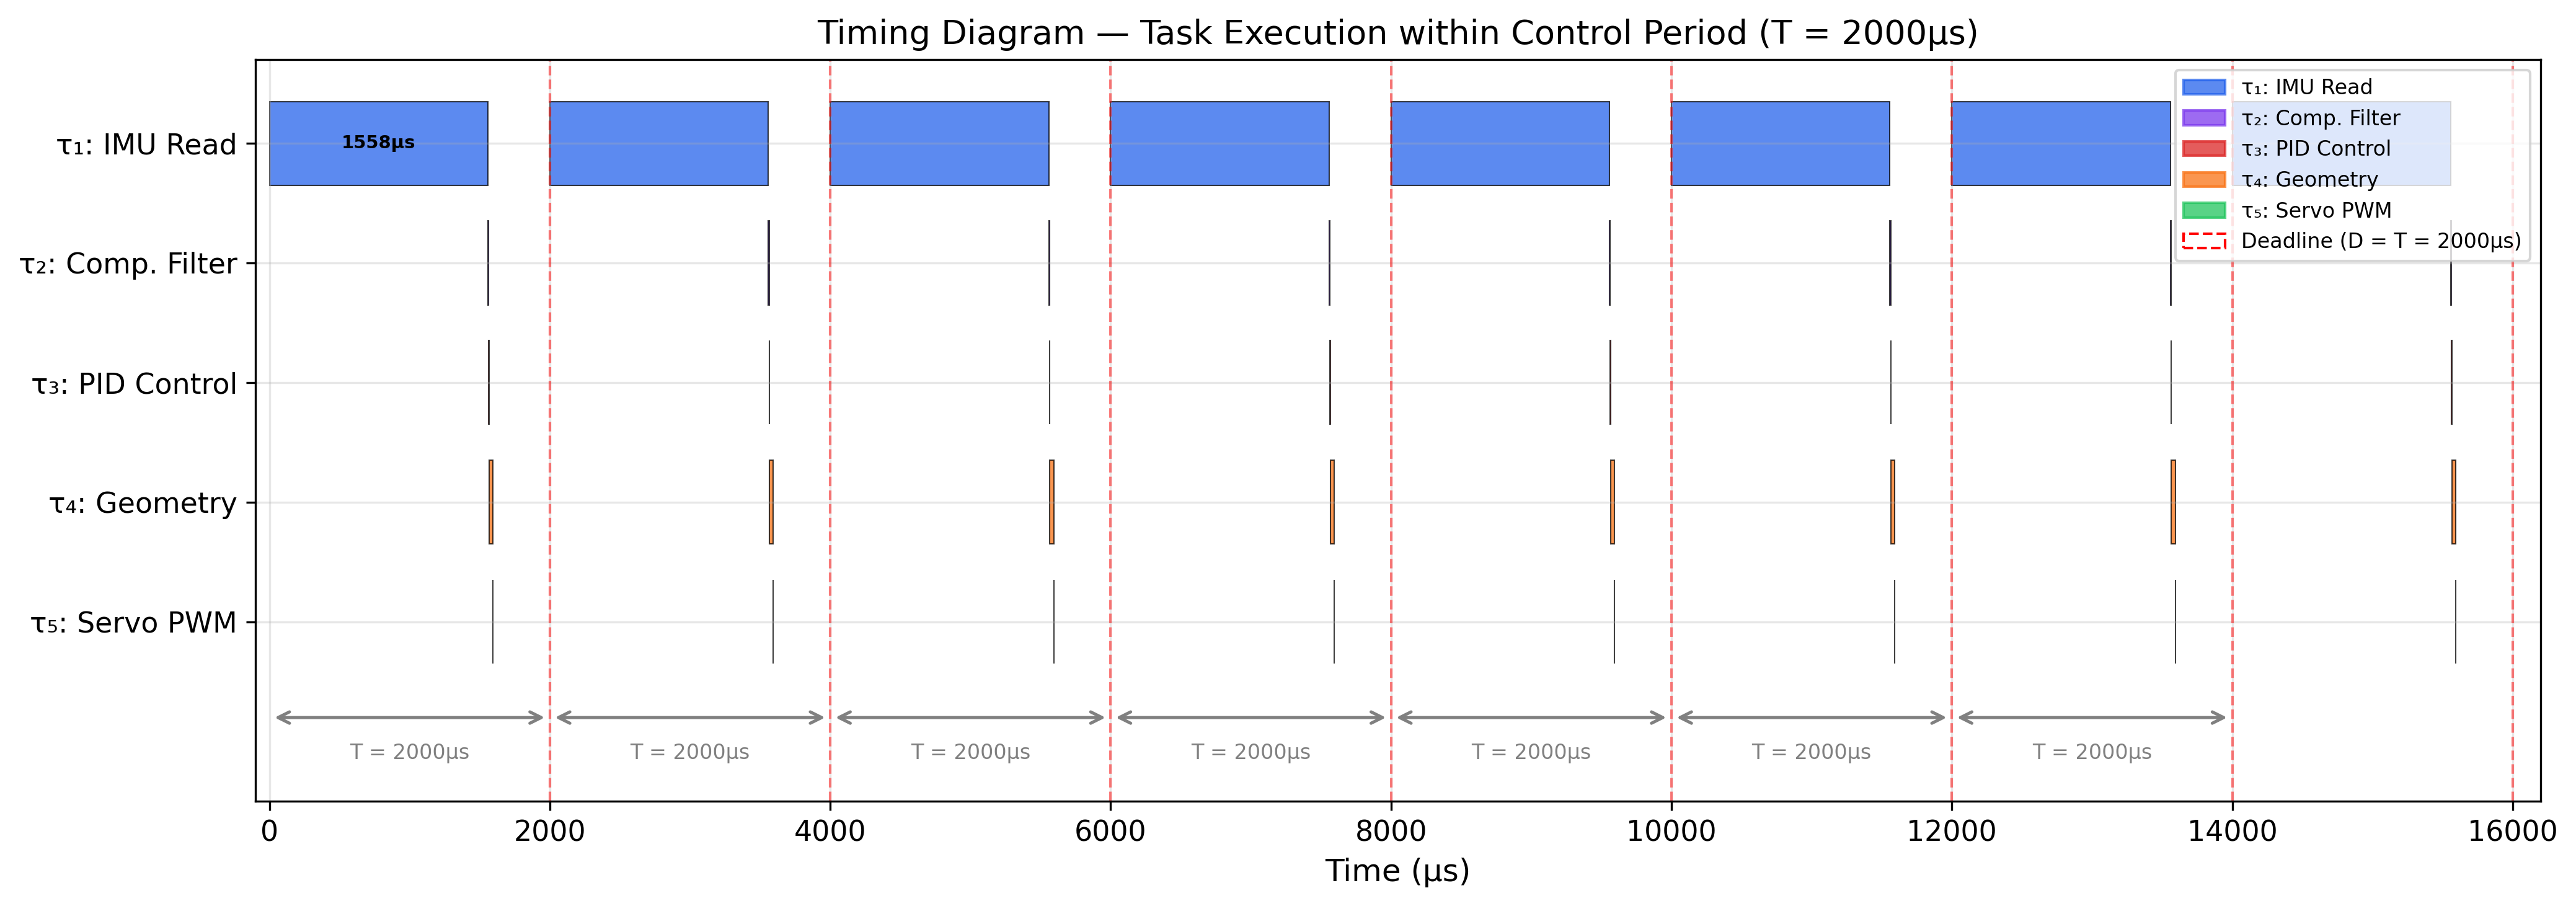
\includegraphics[width=\linewidth]{fig3_timing_diagram.png}
  \caption{Timing diagram over seven consecutive control periods. The IMU read
    $\tau_1$ ($\sim$1563\,$\mu$s) dominates; $\tau_2$--$\tau_5$ are negligible by
    comparison. Every period completes well before the $D=2000\,\mu$s deadline.}
  \label{fig:timing}
\end{figure}

\subsection{Schedulability test}
For a non-preemptive single-rate chain, all tasks must complete within one
period, so the exact (necessary and sufficient) test is simply
$\sum_i C_i \le D$:
\begin{equation}
  1573+7+3+42+4 = 1629\,\mu\text{s} \;\le\; 2000\,\mu\text{s},
\end{equation}
leaving a slack of $D-\sum_i C_i = 371\,\mu\text{s}$ (an 18.6\% margin). Because
execution is sequential, the worst-case response time of the chain equals
$\sum_i C_i = 1629\,\mu\text{s} \le D$, so the system is \textbf{schedulable}.

\paragraph{On the Liu \& Layland bound}
The classical Liu \& Layland utilization bound for $n=5$ preemptive
rate-monotonic tasks is $U \le n(2^{1/n}-1) = 74.3\%$~\cite{liu1973scheduling}.
The measured utilization of $U=81.5\%$ \emph{exceeds} this bound, but the bound does not
apply: it is a \emph{sufficient} test for \emph{preemptive} RM scheduling of
independent periodic tasks, whereas the tasks in this work form a single non-preemptive
sequence sharing one period. For that model, $\sum_i C_i \le D$ is the correct,
exact criterion~\cite{buttazzo2011hard}, and it is satisfied.

\subsection{Empirical verification}
Across all $36{,}031$ logged cycles the firmware recorded \textbf{0 deadline
  misses (0.00\%)}, with observed loop WCET $1614\,\mu$s, mean $1597\,\mu$s, and
P99 $1608\,\mu$s---consistent with the per-task budget. The blocking
I\textsuperscript{2}C read $\tau_1$ consumes 78.6\% of the budget and is the
clear bottleneck; migrating the IMU to SPI ($\sim$400\,$\mu$s) would free
$\sim$1200\,$\mu$s, enough for a substantially faster loop or a true
rate-damping term.

% =====================================================
\section{Stability Analysis}
\label{sec:lyap}
% =====================================================
\subsection{Lyapunov candidate and its derivative}
Consider the state $\mathbf x=[\theta_p,\theta_r]^\top$ with equilibrium
$\mathbf x=\mathbf 0$ (platform level), and the quadratic candidate
\begin{equation}
  V(\mathbf x)=\tfrac12\theta_p^2+\tfrac12\theta_r^2=\tfrac12\lVert\mathbf x\rVert^2.
\end{equation}
$V$ is the squared distance from level (analogous to spring energy
$\tfrac12kx^2$, not literal mechanical energy): $V=0$ when flat, positive and
radially unbounded otherwise. By the chain rule
($\tfrac{d}{dt}\theta^2=2\theta\dot\theta$),
\begin{equation}
  \dot V=\theta_p\,\omega_p+\theta_r\,\omega_r,
  \label{eq:vdot}
\end{equation}
where $\omega=\dot\theta$ is the gyro rate. Equation~\eqref{eq:vdot} has an
intuitive reading: when the platform is tilted and \emph{returning}
($\theta,\omega$ of opposite sign), $\dot V<0$ and things are improving; when it
is tilted and \emph{overshooting} (same sign), $\dot V>0$ and things are
momentarily worsening.

\subsection{Why $\dot V$ cannot be signed analytically}
Lyapunov's direct method certifies asymptotic stability if $\dot V<0$ for
$\mathbf x\ne\mathbf 0$~\cite{khalil2002nonlinear,slotine1991applied}. This cannot
be established analytically for two reasons. First, the controller is
\emph{velocity-form PI}: the $K_d$ term was deliberately dropped
(Section~V), so there is \emph{no explicit rate-damping} that would inject a
guaranteed $-c\,\omega^2$ into \eqref{eq:vdot}. Second, there is no identified
plant model relating $\omega$ to $\theta$ (the string-driven, joint-supported
mechanism with servo dynamics, friction, and string compliance is not modeled).
Consequently, $\dot V=\theta\cdot\omega$ is \emph{not sign-definite}: it is
strictly positive during every overshoot of an under-damped response. Therefore,
asymptotic stability is not claimed analytically; instead, the decrease condition
is verified \emph{quantitatively from logged data} using two
complementary measures.

\subsection{Measure 1: the $\dot V\le 0$ fraction}
The energy change is evaluated sample by sample to determine the fraction of samples for which it is non-increasing:
\begin{equation}
  \rho_{\Delta V}=\frac{1}{M-1}\sum_{k=0}^{M-2}
  \mathbf 1\!\big[\,V[k{+}1]-V[k]\le 0\,\big]\times 100\%,
\end{equation}
where $\mathbf 1[\cdot]$ is the indicator function. Since
$\dot V\approx (V[k{+}1]-V[k])/\Delta t$ with $\Delta t>0$, this yields
$\operatorname{sign}(\Delta V)=\operatorname{sign}(\dot V)$, hence $\rho_{\Delta V}$
is exactly the fraction of time the Lyapunov decrease condition $\dot V\le 0$
holds---it tests the \emph{direction} of the energy change, not its speed.

\paragraph{Interpreting $\rho_{\Delta V}\approx 50\%$}
The experimental data yield an average of $\rho_{\Delta V}=49.7\%$. This is \emph{not} a sign of
instability but the \textbf{signature of an under-damped oscillation}: energy
\emph{rises} during overshoot (about half the time) and \emph{falls} during the
return (about half), like a swing whose height goes up and down on each pass
even as its peaks shrink. A per-sample count near $50\%$ therefore indicates that the
system oscillates; whether it \emph{converges} must be judged from the
\emph{envelope} of the peaks, which is what the second measure does.

\subsection{Measure 2: the decay rate $\gamma$}
The stronger, quantitative stability condition is that the energy decays
proportionally to itself,
\begin{equation}
  \dot V\le-\gamma V,\qquad\gamma>0.
  \label{eq:gammacond}
\end{equation}
Solving the equality case as a first-order linear ODE,
\begin{equation}
  \frac{dV}{dt}=-\gamma V
  \;\Rightarrow\;\frac{dV}{V}=-\gamma\,dt
  \;\overset{\textstyle\int}{\Longrightarrow}\;\ln V=-\gamma t+\text{const}
  \;\Rightarrow\;V(t)=V_0\,e^{-\gamma t},
\end{equation}
which is exponential decay with time constant $\tau=1/\gamma$---the same form as
a damped spring, an RC discharge, or Newtonian cooling, where $V_0$ is the
energy at the onset of a disturbance. Taking logarithms linearizes it,
$\ln V(t)=\ln V_0-\gamma t$. Therefore, $\gamma$ is extracted for each disturbance event
by fitting a straight line to the \emph{peak envelope} of $\ln V$ (a moving-max
envelope, so noise valleys do not bias the slope) and reading
\begin{equation}
  \gamma=-\,\text{slope of }\ln V_\text{peak}\ \text{vs }t.
\end{equation}
The interpretation is direct: $\gamma>0$ means $V$ decays (the envelope shrinks,
the system converges); $\gamma=0$ means a sustained oscillation; $\gamma<0$
means $V$ grows (unstable). The two measures are complementary:
$\rho_{\Delta V}$ tests whether energy decreases \emph{often}, while $\gamma$
tests whether it decreases \emph{on the whole}. An under-damped but stable
system has $\rho_{\Delta V}\approx 50\%$ \emph{and} $\gamma>0$, which corresponds
to the behavior of the proposed system.

\subsection{Results}
A quantitative analysis was applied to the $80\,\text{s}$, $36{,}031$-sample log,
which contains four disturbance events (Fig.~\ref{fig:lyap}). The per-event
results are in Table~\ref{tab:lyap}. The energy is bounded throughout
($V_{\max}=45.3<\infty$, no escape), every event's envelope decays
($\gamma>0$), and the average decay rate is $\gamma=0.275\,\text{s}^{-1}$
($\tau\approx3.6\,$s). The $\dot V\le0$ fraction sits at $49.7\%$, confirming the
under-damped-but-converging picture.

\begin{table}[t]
  \caption{Per-Event Quantitative Stability Measures}
  \label{tab:lyap}
  \centering
  \small
  \begin{tabular}{ccccc}
    \toprule
    Event        & $V_\text{peak}$ & $\gamma$ (s$^{-1}$) & $\tau$ (s)   & $\rho_{\Delta V}$ \\
    \midrule
    \#1          & 22.45           & 0.158               & 6.3          & 49.1\%            \\
    \#2          & 45.29           & 0.317               & 3.2          & 49.7\%            \\
    \#3          & 42.11           & 0.304               & 3.3          & 48.9\%            \\
    \#4          & 27.62           & 0.320               & 3.1          & 51.0\%            \\
    \midrule
    \textbf{avg} & ---             & \textbf{0.275}      & \textbf{3.6} & \textbf{49.7\%}   \\
    \bottomrule
  \end{tabular}
\end{table}

\begin{figure}[t]
  \centering
  
\includegraphics[width=\linewidth]{fig7_lyapunov.png}
  \caption{Empirical Lyapunov function. Top: tilt magnitude
    $\lVert\mathbf x\rVert$ with the steady-state RMS line; dotted markers are
    disturbance onsets. Bottom: $V(t)=\tfrac12\lVert\mathbf x\rVert^2$ with the
    ultimate-bound level $V_\infty=5.71$. After each disturbance, $V$ spikes and
    then decays back into the residual ball.}
  \label{fig:lyap}
\end{figure}

\subsection{Ultimate bound and verdict}
The trajectory does not converge to $0$ but to a residual ball. From the last
20\% of the log, the steady-state RMS tilt is $3.38^\circ$ (max $7.43^\circ$),
giving an ultimate bound $V_\infty=\tfrac12(3.38^\circ)^2 = 5.71$, i.e.\ a ball
of radius $\sim$$3.4^\circ$. Combining the three facts---(i) $V$ is bounded,
    (ii) the post-disturbance envelope decays with $\gamma=0.275\,\text{s}^{-1}$,
    and (iii) the trajectory settles into a $\sim$$3.4^\circ$ ball---the platform is
  \textbf{practically stable / ultimately bounded}~\cite{khalil2002nonlinear}, not
  asymptotically stable to $0$. The nonzero residual is the expected price of the
  soft deadband, the leaky integrator, sensor noise, and---most importantly---the
  absence of an explicit velocity-damping term, which is exactly what the
  under-damped $\rho_{\Delta V}\approx50\%$ signature predicts.

  % =====================================================
  \section{Experimental Results}
  % =====================================================
  Fig.~\ref{fig:step} shows the closed-loop step response on both axes over the
$80\,\text{s}$ run. The platform absorbs peak disturbances of $\sim$$8.2^\circ$
  and recovers consistently to the $\pm1^\circ$ band, with an average settling
  time of $11.96\,$s (a slow recovery that is a direct consequence of the missing
  damping term and the low PI gains chosen for vibration robustness). The
  steady-state RMS tilt is $3.38^\circ$. Table~\ref{tab:summary} consolidates the
  real-time and control metrics.

  \begin{figure}[t]
    \centering
    
\includegraphics[width=\linewidth]{fig1_step_response.png}
    \caption{Closed-loop step response (pitch and roll) across four disturbance
      events. The platform returns to the $\pm1^\circ$ settled band after each push.}
    \label{fig:step}
  \end{figure}

  \begin{table}[t]
    \caption{Performance Summary}
    \label{tab:summary}
    \centering
    \small
    \begin{tabular}{ll}
      \toprule
      \textbf{Real-time}            &                                              \\
      \midrule
      Control frequency             & 500\,Hz ($T=2000\,\mu$s)                     \\
      WCET ($\sum_i C_i$)           & $1629\,\mu$s ($<2000\,\mu$s)                 \\
      CPU utilization               & 81.5\%                                       \\
      Deadline margin               & 18.6\%                                       \\
      Deadline miss rate            & 0.00\% (0/36{,}031)                          \\
      \midrule
      \textbf{Control \& stability} &                                              \\
      \midrule
      Avg.\ settling time           & 11.96\,s                                     \\
      Steady-state RMS tilt         & $3.38^\circ$                                 \\
      Lyapunov $V$                  & bounded ($V_{\max}=45.3$)                    \\
      Decay rate $\gamma$           & $0.275\,\text{s}^{-1}$ ($\tau\approx3.6$\,s) \\
      Stability class               & practical / ultimately bounded               \\
      \bottomrule
    \end{tabular}
  \end{table}

  % =====================================================
  \section{Conclusion and Future Work}
  % =====================================================
  A complete cyber-physical control loop---IMU $\rightarrow$
  complementary filter $\rightarrow$ velocity-form PI $\rightarrow$ exact
  string-length inverse kinematics $\rightarrow$ PWM---was built and verified for a self-stabilizing
  adaptive tray. The inverse-kinematic model, derived from a rigid-body rotation
  about the central joint, turns a desired tilt angle into the precise string
  length and servo rotation each actuator must produce, avoiding the nonlinear
  failure of a direct angle mapping. The task set is provably and empirically
  schedulable at 500\,Hz ($1629 \le 2000\,\mu$s, 0 deadline misses over
$36{,}031$ cycles). Because the controller has no explicit damping term and no
  identified plant model, stability was certified quantitatively from data: the
  Lyapunov energy is bounded and its post-disturbance envelope decays at
$\gamma=0.275\,\text{s}^{-1}$, while the $\dot V\le0$ fraction near $50\%$
  correctly flags an under-damped---but converging---response that settles into a
$\sim\!3.4^\circ$ ball (practical / ultimate boundedness).

  The analysis points directly to the next steps. Moving the IMU from
  I\textsuperscript{2}C to SPI removes the dominant $\sim$1200\,$\mu$s of
$\tau_1$, freeing budget for (i) a faster loop and (ii) a genuine gyro-rate
  damping term, which would inject the missing $-c\,\omega^2$ into $\dot V$,
  shrink the residual ball, and cut the settling time. Systematic $K_P,K_I$
tuning and a Kalman attitude filter are natural further improvements.

\section*{Acknowledgment}
The authors thank Prof.~Chao Wang for guidance throughout the CSC9008
Cyber-Physical Systems course, and Chiin~H.\ for assistance with the mechanical
build.

\bibliographystyle{IEEEtran}
\bibliography{references}

\end{document}
